%Praca inżynierska (c) Kamil Strzempowicz
\documentclass[twoside]{kInzynierka}
\usepackage{polski}
%\usepackage[polish]{babel}
\usepackage[utf8]{inputenc}
\usepackage{mathtools}
\usepackage{color}
\usepackage{graphicx}
\usepackage{transparent}
\usepackage{lscape}
\usepackage[section]{placeins}
\usepackage[justification=raggedright,singlelinecheck=false,labelsep=period]{caption}
%hyperref musi być ostatnie
%\usepackage[hidelinks]{hyperref}
\usepackage{hyperref}
%%%%%%%%%%%%%%%%%%%%%%%%%%
%%% Przełączniki stylu %%%
%%%%%%%%%%%%%%%%%%%%%%%%%%

%\mathtoolsset{showonlyrefs}
%\sectionWzory  
%\drukJednostronny
%\literowaNumeracjaDodatkow %% w³¹czy numeracjê dodatków literami


%%%%%%%%%%%%%%%%%%%%%%%
%%% Podstawowe info %%%
%%%%%%%%%%%%%%%%%%%%%%%

\title{Strategia Just in Time w systemach produkcyjnych\\ - analiza struktury gniazdowej dla heurystyk FIFO i LIFO.}
\promotor{dr inż. Waldemar Grzechca}
\autor{Kamil Strzempowicz}{100}{Napisanie całej pracy}
\dedykacja{Rodzicom\\bez Was nie udałoby mi się}

%%%%%%%%%%%%%%%%%%%%%%%%%%%%%%%%%
%%% początek właściwej treści %%%
%%%%%%%%%%%%%%%%%%%%%%%%%%%%%%%%%

\begin{document}
\section        {Wstęp}
Celem tej pracy jest przedstawienie strategii Just in Time dla szeregowania zadań w systemach produkcyjnych o strukturze gniazdowej. Szeregowanie przeprowadzono na podstawie heurystyk First In First Out i Last In First Out. Na potrzeby tej pracy powstał program \emph{kSzereg} szeregujący zadania według heurystyk FIFO i LIFO, oraz obliczający wyznaczniki jakosci uszeregowania w kontekście strategii JIT.

System produkcyjny jest to celowo zaprojektowany i zorganizowany układ materialny, energetyczny i informacyjny eksploatowany przez człowieka i służący produkowaniu określonych produktów (wyrobów lub usług) w celu zaspokajania różnorodnych potrzeb konsumentów. \cite{pastuszak}
Systemy produkcyjne można podzielić ze względu na strukturę na:
\begin{itemize}
\item Systemy gniazdowe - zwykle wykorzystywane do pojedyńczych zamówień, bądź krótkich serii. Takie systemy zwykle zmieniają swoje zastosowanie po zakończeniu każdego zlecenia. Zlecenie składa się ze skończonej liczby zadań, a każde z nich wymaga przeprowadzenia zestawu operacji na maszynach w ustalonym porządku, innym dla każdego zadania.
\item System przepływowy - Kierunek przepływu wszystkich zleceń przez maszyny jest ten sam. Dla idealnego systemu przepływowego liczba zadań jest równa liczbie maszyn dla każdego zlecenia. \cite{grzechca}
\item Pojedyńcza maszyna - system składający się z jednej tylko maszyny. Zakłada się, że procesy wytwarzania produktów są jednostadialne, a zlecenia jednostkowe. Stąd zlecenia są tożsame z zadaniami, przy czym nie istnieją ograniczenia kolejnościowe. \cite{grzechca}
\item Maszyny równoległe - system składający się z m identycznych maszyn. Podobnie jak w problemie jednomaszynowym zakłada się, że procesy wytwarzania produktów są jednostadialne, a zlecenia jednostkowe. Stąd, podobnie jak tam, zlecenia są tożsame z zadaniami, przy czym nie istnieją ograniczenia kolejnościowe. \cite{grzechca}
\item Linia montażowa -  zespół stanowisk roboczych (maszynowych, ręcznych lub mieszanych) ugrupowanych według kolejności operacji procesu technologicznego. \cite{wiki}
\end{itemize}

Szeregowanie może zostać zdefiniowne jako przydział zasobów w czasie do zadań w celu optymalizacji kryterium. Z punktu widzenia szeregowania w systemach wytwarzania zasoby często są nazywane maszynami, natomiast jako kryterium optymalności uszeregowania często przyjmowany jest czas potrzebny do zakończenia wszystkich zadań, czy maksymalne spóźnienie zadania. \cite{antColony}  

W strategi Just in Time zadanie powinno być ukończone możliwie blisko swojego terminu zakończenia (due date) jak to tylko możliwe. Zbyt wczesne zakończenie zadania pociąga za sobą koszty utrzymania, takie jak magazynowania czy ubezpieczenia. Z drugiej jednak strony spóźnione zlecenie często skutkuje karami umownymi czy nadszarpnięciem reputacji przedsiębiorstwa. Mimo to często przedsiębiorstwu bardziej opłaca się zakończyć zadanie krótko po terminie, niż ponosić koszty związane ze zbyt wczesnym zakończeniem pracy. Należy się więc zastanowić jak matematycznie opisać opłacalność zarówno spóźnienia jak i przedwczesnego ukończenia zadania. Taką rolę pełnią tzw. funkcje kosztu. \cite{genetyczne} Na potrzeby tej pracy wybrano następujące funkcje:

\begin{equation}
    \sqrt{(\sum e_j^2 + \sum l_j^2}
    \label{eq:w1}
\end{equation}
\begin{equation}
    \alpha*\sum e_j + \beta*\sum l_j
    \label{eq:w2}
\end{equation}
, gdzie \\
\(e_j\) - przedwczesność j-tego zadania, \\
\(l_j\) - spóźnienie j-tego zadania, \\
\(\alpha, \beta\) - wagi przedwczesności i spóźnienia zakładane przy formuowaniu problemu\\

Zastosowanie strategi Just in Time w systemach produkcyjnych o strukturze gniazdowej można więc sprowadzić do poszukiwania takiego rozwiązania problemu harmonogramowania, aby minimalizować funckję \ref{eq:w1} lub \ref{eq:w2}.

\section        [Metody szeregowania zadań \ldots]
		        {Metody szeregowania zadań \newline w systemach wytwarzania gniazdowego}

Teoretycznie optymalne rozwiązanie problem szeregowania zadań w systmie wytwarzania gniazdowego (skr. JSSP) można dokonać na podstawie przeglądu zupełnego, ponieważ zawsze ilość możliwych rozwiązań zawsze jest skończona. Jednak problem ten jest silnie NP-trudny, czyli pozaostaje NP-trudny nawet przy ograniczeniu maksymalnej wartości występujących w jego opisie liczb. Natomiat problem NP-trudny jest co najmniej tak trudny jak każdy problem klasy NP (nondeterministic polynomial), a często trudniejszy. Oznacza to, że już przy niewielkiej ilości zadania problem przestaje być rozwiązywalny w rozsądnym czasie nawet przy użyciu superkomputerów. W związku z tym wykorzystuje się metody pozwalające uzyskać nieoptymalne, ale akceptowalne rozwiązanie bez potrzeby rozpatrywania każdego możliwego rozwiązania. \cite{np}

\subsection     {Metody heurystyczne}
Metody heurystyczne pozwalają na stosunkowo szybkie i łatwe znalezienie dopuszczalnego rozwiązania. Zwykle jednak nie jest to rozwiązanie optymalne, lecz niejednokrotnie bardziej opłacalne jest wdrożenie takiego rozwiązania, niż żmudne poszukiwanie lepszego rozwiązania, ze względu na czas i zasoby wymagane do jego odnalezienia. W szczególności w sytuacji awaryjnej, gdy nie ma czasu na wykorzystanie bardziej zaawansowanych metod. 

Metody te zwykle polegają na nadawaniu priorytetu, na podstawie danych zlecenia i chwili czasu, zadaniom w momencie wystąpienia konflktu. Konflikt jest to sytuacja gdy w tym samym momencie na dany wolny zasób (maszynę) czeka więcej niż jedno zadanie. Trzeba wtedy zdecydować które z zadań zostanie obsłużone jako pirwsze. 

Najpopularniejsze heurystyki:
\begin{itemize}
\item First In First Out - Pierwsze jest przetwarzane zadanie które wpłynęło najwcześniej.
\item Last In First Out - Pierwsze jest przetwarzane zadanie które wpłynęło najpóźniej.
\item Earliest Due Date - Pierwsze jest przetwarzane zadanie które ma zostać wyprodukowane najwcześniej.
\item Least Work Remaining - Pierwsze jest przetwarzane zadanie do ukończenia którego pozostało najmniej pracy.
\item Shortest Procesing Time - Pierwsze jest przetwarzane zadanie którego całkowity czas przetwarzania jest najkrótszy.
\item Longest Procesing Time - Pierwsze jest przetwarzane zadanie którego całkowity czas przetwarzania jest najdłuższy.
\item Shortest Imminent Procesing Time - Pierwsze jest przetwarzane zadanie którego czas przetwarzania na tej maszynie jest najkrótszy.
\item Longest Imminent Procesing Time - Pierwsze jest przetwarzane zadanie którego czas przetwarzania na tej maszynie jest najdłuższy.
\item Fewest Operationns Remmaining - Pierwsze jest przetwarzane zadanie do ukończenia którego potrzeba najmniejszej ilości operacji.
\item Most Operationns Remmaining - Pierwsze jest przetwarzane zadanie do ukończenia którego potrzeba największej ilości operacji.
\item Least Slack Time - Pierwsze jest przetwarzane zadanie którego różnica między czasem potrzebnym do jego ukończenia a czesem pozostałym do terminu zakończenia pracy jest najmniejsza.
\item Least Slack Time per Operation - Pierwsze jest przetwarzane zadanie którego stosunek czasu 'Slack' w
\item Critical Ratio - Pierwsze jest przetwarzane zadanie którego stosunek czasu pozostałego do terminu ukończenia pracy i czasu potrzebnego do jego ukończenia jest najmniejszy.
\item Random - Losowe zadanie jest przetwarzane jako pierwsze.
\end{itemize}

\subsection     {Inne metody}
Istnieją też nieheurystyczne metody szeregowania zadań w systemach wytwarzania gniazdowego. Zwykle wymagają one więcej czasu i zasobów niż metody heurystyczne, jednocześnie nie gwarantują uzyskania lepszego rozwiązania. Na przykład metoda podziałów i oszacowań, która pozwala 'odciąć' nieoptymalne gałęzie z grafu wszystkich rozwiązań i pozwala na znalezienie rozwiązania optymalnego, jednak przy wielu zadaniach trwa to na tyle długo, że zwykle po znalezieniu satysfakcjonującego rozwiązania algorytm jest przerywany.

Do znalezienia rozwiązania JSSP można wykorzystać także algorytmy genetyczne, które są adaptacyjnym narzędziem ukierunkowanego poszukiwania optimum funkcji celu (np. \ref{eq:w1}, czy \ref{eq:w2}), które pozwala na równoległe przeszukiwanie zakodowanej przestrzeni alternatywnych rozwiązań. Procedura ta wykorzystuje procesy losowe do określenia kierunku przeszukiwania. Idea algorytmów genetycznych naśladuje zasadę działania rzeczywistego mechanizmu ewolucyjnego, czyli darwinowską strategię przetrwania osobników biologicznie najlepiej przystosowanych. Możemy zasymulować ten proces i zastosować go do rozwiązywania problemów trudnych obliczeniowo, dla których nie jesteśmy w stanie skonstruować algorytmu dającego dokładne rozwiązanie w rozsądnym czasie (problemy klasy NP), przy czym w ogólnym przypadku uzyskujemy rozwiązania suboptymalne, za to stosunkowo szybko. Dodatkowo wyniki działania algorytmu genetycznego można poprawić stosując Lokalne Poszukiwanie. \cite{grzechca} \cite{genetyczne}

%\newlineTekst
%\newlineSpis
\section        [Heurystyki FIFO i LIFO \ldots]
                {Heurystyki FIFO i LIFO w JSSP \newlineTekst - przykład obliczeniowy}
Algorytm rozwiązywania problemu szeregowania zadań w systemie wytwarzania gniazdowego za pomocą heurystyk FIFO i LIFO ilustruje poniższy przykład. Dane zlecenia zostały przedstawione w formie tabeli, gdzie: \\
j - numer zadania \\
\(r_j\) - czas pojawienia się zadania w systemie \\
\(d_j\) - termin ukończenia zadania \\
m1-m5 - numer maszyny na której zadanie ma być przetwarzane w czasie zapisanym w nawiasie.
\begin{table}[htb]
	\centering
	\begin{tabular}{ | r | c | c | l | }
	\hline
	j	& \(r_j\)	& \(d_j\)	& Marszruta technologiczna	\\ \hline
	1	& 0	& 20	& m4 (4) - m2 (6) - m4 (5)	\\ \hline
	2	& 3	& 29	& m4 (3) - m3 (6) - m1 (5) - m4 (5)	\\ \hline
	3	& 0	& 20	& m1 (5) - m5 (4)	\\ \hline
	4	& 0	& 20	& m5 (4) - m1 (4) - m2 (6)	\\ \hline
	5	& 3	& 20	& m1 (3) - m5 (4)	\\ \hline
	\end{tabular}
	\caption{Struktura zlecenia}
\end{table}

\begin{table}[htb]
    \begin{tabular}{ p{0.75cm} | p{13cm} }
    t & Zdarzenie \\ \hline
    0 & Do systemu wchodzą zadania 1, 3 i 4 które zostają przydzielone zgodnie ze swoimi marszrutami technologicznymi odpowiednio do maszyn m4, m1 i m5.  \\ \hline
    3 & Do systemu wchodzą zadania 2 i 5, lecz maszyny na których powinno zacząć się ich przetwarzanie są zajęte, czekają więc na zwolnienie maszyny. \\ \hline
    4 & Na maszynie 5 zakończyło się przetwarzanie zadania 4. Na tę maszynę żadne zadanie nie oczekiwało. Na maszynie 4 zakończyło się przetwarzanie zadania 1. Na tę maszynę oczekuje tylko zadanie 2, które zostaje od razu na niej uruchomione. Zadanie 1 natomiast czeka na zwolnienie się maszyny 1. \\ \hline
    5 & Przetwarzanie zadanie 3 na maszynie 1 dobiegło końca. Na tę maszynę oczekiwały dwa zadania: 1 i 5, więc nastąpił tzw. konflikt.   
    \end{tabular}
    \caption{Algorytm szeregowania zadań - cz.1}
\end{table}

\begin{figure}[htb]
    \centering
    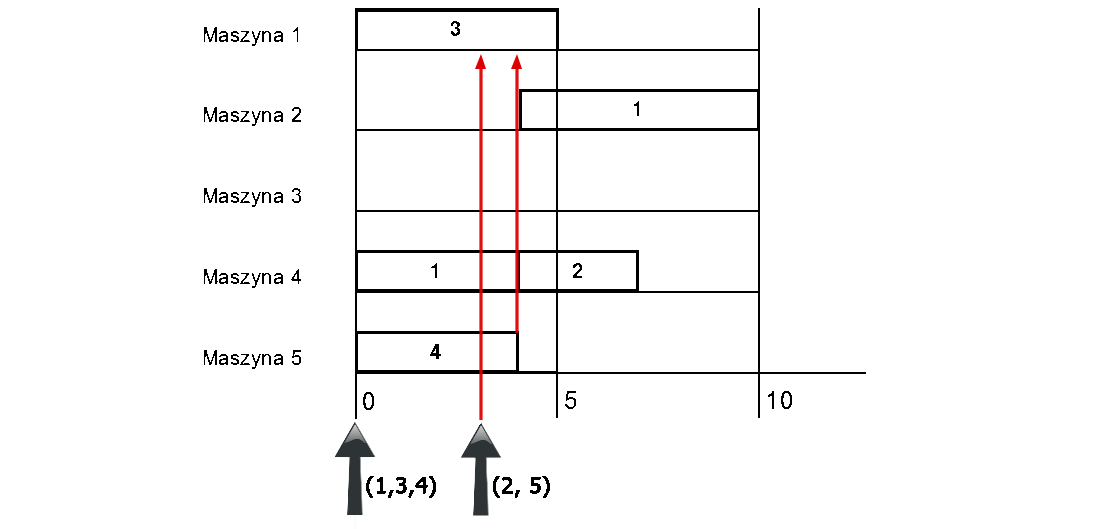
\includegraphics[width=\textwidth, keepaspectratio=true]{./obrazki/konf}
    \caption{Uszeregowanie zadań w chwili wystąpienia konfliktu}
\end{figure}

Heurystyki służą do rozwiązywania takich właśnie konfliktów. Jeżeli zdecydujemy się na heurystykę FIFO dostęp do maszyny uzyska to zadanie które oczekuje najdłużej (jako pierwsze "zajęło miejsce w kolejce"), w tym przypadku jest to zadanie 5. Heurystyka LIFO faworyzuje zadania najkrócej oczekujące na zasób, w tym przypadku więc będzie to zadanie 4. Jeżeli nastąpiłby konflikt między dwoma równoprawnymi pod względem wybranej heurystyki zadaniami, należy wtedy zastosować dowolną inną "pomocniczą" heurystykę, choćby Random, czyli wybranie losowego zadania.

Dalsze rozwiązanie tego przykładu krok po kroku nie zostanie tu zaprezentowane, natomiast końcowe uszeregowanie w zależności od wybranej heurystyki przedstawiają poniższe wykresy Gantt'a oraz wyznaczniki jakości uszeregowania. Różnice między tymi dwoma uszeregowaniami wydają się być kosmetyczne, wynika to jednak z trywialności omawianego przykładu. Podczas analizy tych wyznaczników widać różnice między uszeregowaniami. W tym konkretnym przypadku wybór heurystyki nie wpłyną na \(C_max\), czyli czas ukończenia całego zlecenia. Jednak trochę lepsze rozwiązanie, ze względu na \(\bar{F}\) oraz \(\sqrt{(\sum e_j^2 + \sum l_j^2}\), dała heurystyka FIFO.

\FloatBarrier
\subsection{First In First Out}

\begin{figure}[htb]
    \centering
    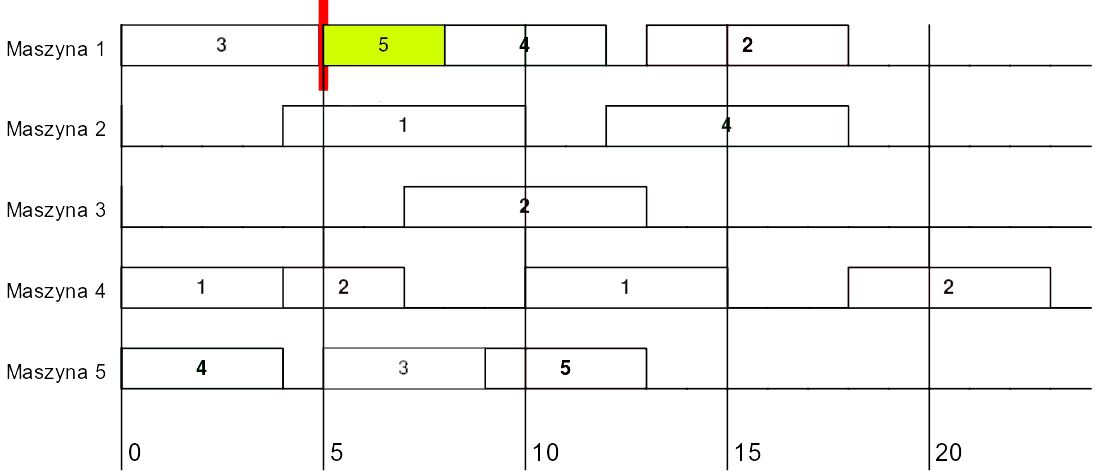
\includegraphics[width=\textwidth, keepaspectratio=true]{./obrazki/fifo}
    \caption{Uszeregowanie przy użyciu heurystyki FIFO}
\end{figure}
\begin{table}[htb]
    \centering
    \begin{tabular}{ l l }
    \(C_{max} = 23 \)	& \(\sqrt{(\sum e_j^2 + \sum l_j^2} = 15.3297\)	\\
    \(\bar{F} = 15.6 \)	& \( \alpha*\sum e_j + \beta*\sum l_j \Big|_{\substack{\alpha = 0\\ \beta = 0}} = 0 \)	\\ 
    \end{tabular}
    \caption{Wyznaczniki jakości uszeregowania}
\end{table}
	
\FloatBarrier
\subsection{Last In First Out}

\begin{figure}[htb]
    \centering
    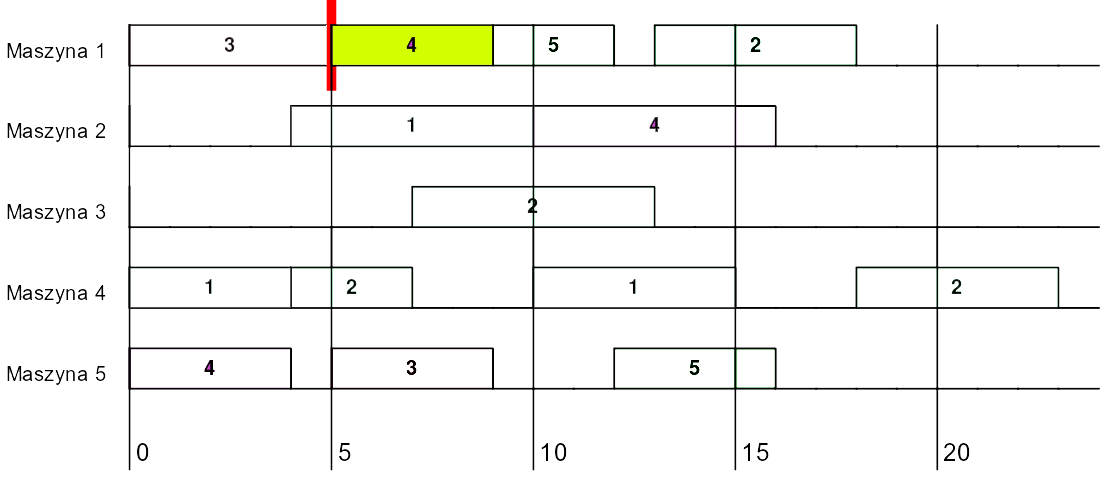
\includegraphics[width=\textwidth, keepaspectratio=true]{./obrazki/lifo}
    \caption{Uszeregowanie przy użyciu heurystyki LIFO}
\end{figure}
\begin{table}[htb]
	\centering
	\begin{tabular}{ | r | c | c | c | c |}
	\hline
	j	& \(c_j\)	& \(f_j\)	& \(l_j\)	& \(e_j\)	\\ \hline
	1	& 18	& 18	& 0	& 2	\\ \hline
	2	& 23	& 23	& 0	& 6	\\ \hline
	3	& 12	& 12	& 0	& 8	\\ \hline
	4	& 19	& 19	& 0	& 1	\\ \hline
	5	& 8	& 8	& 0	& 12	\\ \hline
	\end{tabular}
	\caption{Parametry wykonanych zadań}
\end{table}
       
\section        {Program kSzereg}
%\subsection     {Front-end}
Program kSzereg został napisany w C++ na potrzeby tej pracy dyplomowej. Umożliwia on przeprowadzenie szeregowania zadań w systemie wytwarzania gniazdowego na podstawie heurystyki FIFO bądź LIFO. Wprowadzanie danych odbywa się za pośrednictwem graficznego interface'u opartego o framework Qt. Na górnej belce programu po prawej stronie znajdują się kontroli umożliwiające wybór heurystyki używanej do rozwiązania zadania oraz parametrów \(\alpha, \beta\) podstawianych do wzoru \eqref{eq:w2}. Znajdują się tam też przyciski umożliwiające zapisanie zlecenia da pliku binarnego z rozszerzeniem .mar (eksport), oraz wczytanie zleenia z takiego pliku (import). 

Przed dodaniem zadań do zlecenia należy ustalić maksymalną długość marszruty. W zadaniach z krótszą marszrutą technologiczną należy pozostawić operacje z zerowym czasem, które nie będą brane pod uwagę podczas rozwiązywania JSSP. Po dodaniu zadania możliwość zmiany długości marszruty jest blokowana. Każda operacja jest definiowana prze numer maszyny na której ma zostać wykonana oraz czas jej wykonywania. Ilość maszyn możliwych do wyboru może być zmieniana w czasie edycji zlecenia (po dodaniu zadań). Poza marszrutą technologiczną zadanie definiują czasy rozpoczęcia (\(r_j\)) i zakończenia (\(d_j\)) zadania. Możliwe jest też nadanie zadaniu nazwy.

\begin{figure}[htb]
    \centering
    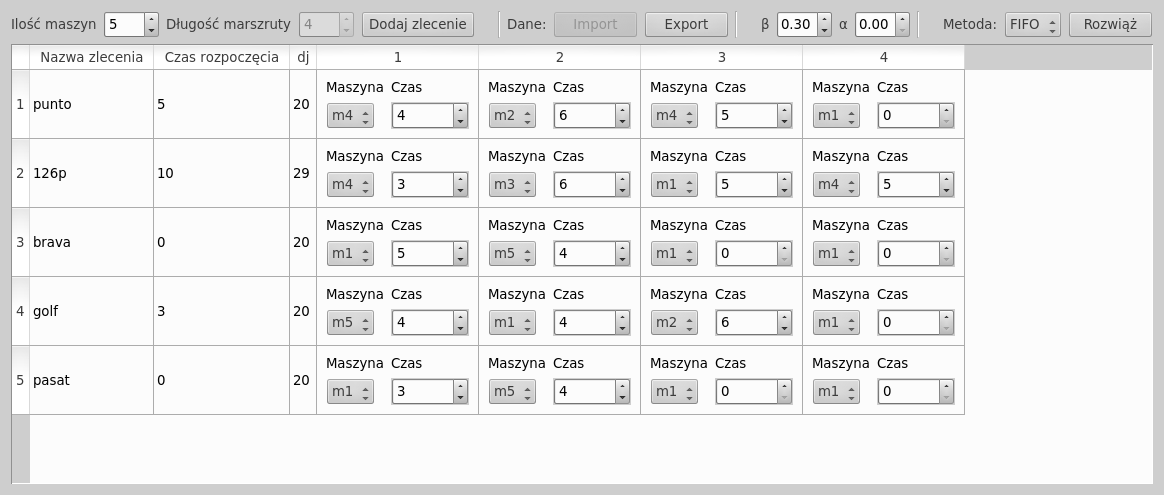
\includegraphics[width=\textwidth, keepaspectratio=true]{./obrazki/main}
    \caption{Główne okno programu}
\end{figure}

Program kSzereg rezentuje wyniki działania w postaci wykresu Gantt'a wraz z tabelą zawierającą czasy wykonania (\(C_j\)), przepływu (\(f_j\)), spóźnienia (\(l_j\)) i przedwczesności (earliness, \(e_j\)) każdego zadania zlecenia. Dodatkowo prezentowane są wyznaczniki jakości uszeregowania zlecenia jako cołości: czas ukończenia całego zadania (\(C_{max}\)), średni czas przepływu (\( \bar{F} \)), oraz wartości funkcji kosztów \eqref{eq:w1} oraz \eqref{eq:w2} opisanych we wstępie do niniejszej pracy. 

\begin{figure}[htb]
    \centering
    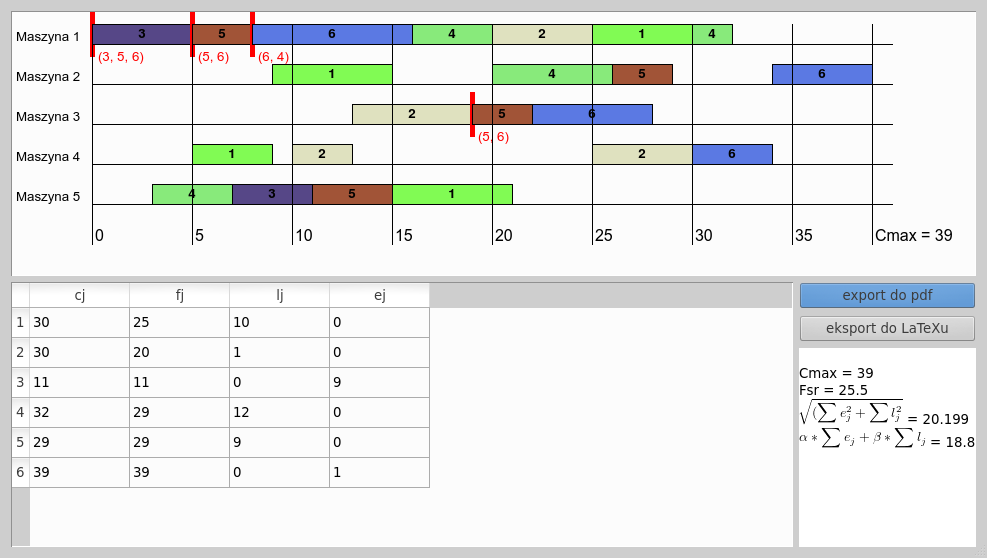
\includegraphics[width=\textwidth, keepaspectratio=true]{./obrazki/wykres}
    \caption{Prezentacja wyznaczonego uszeregowania}
\end{figure}

Z poziomu okna wyznaczonego uszeregowania istnieje możliwość zapisania wyników działania programu w postaci pliku .tex z kodem \LaTeX{}'a lub .pdf. W obu przypadkach sam wykres Gantt'a jest eksportowany do pliku .svg w folderze output. Opcje te korzystają jednak z zewnętrznych programów inkscape oraz rubber (wraz z odpowiednimi paczkami texlive), które muszą być zainstalowane w systemie. 

\begin{figure}[htb]
    \centering
    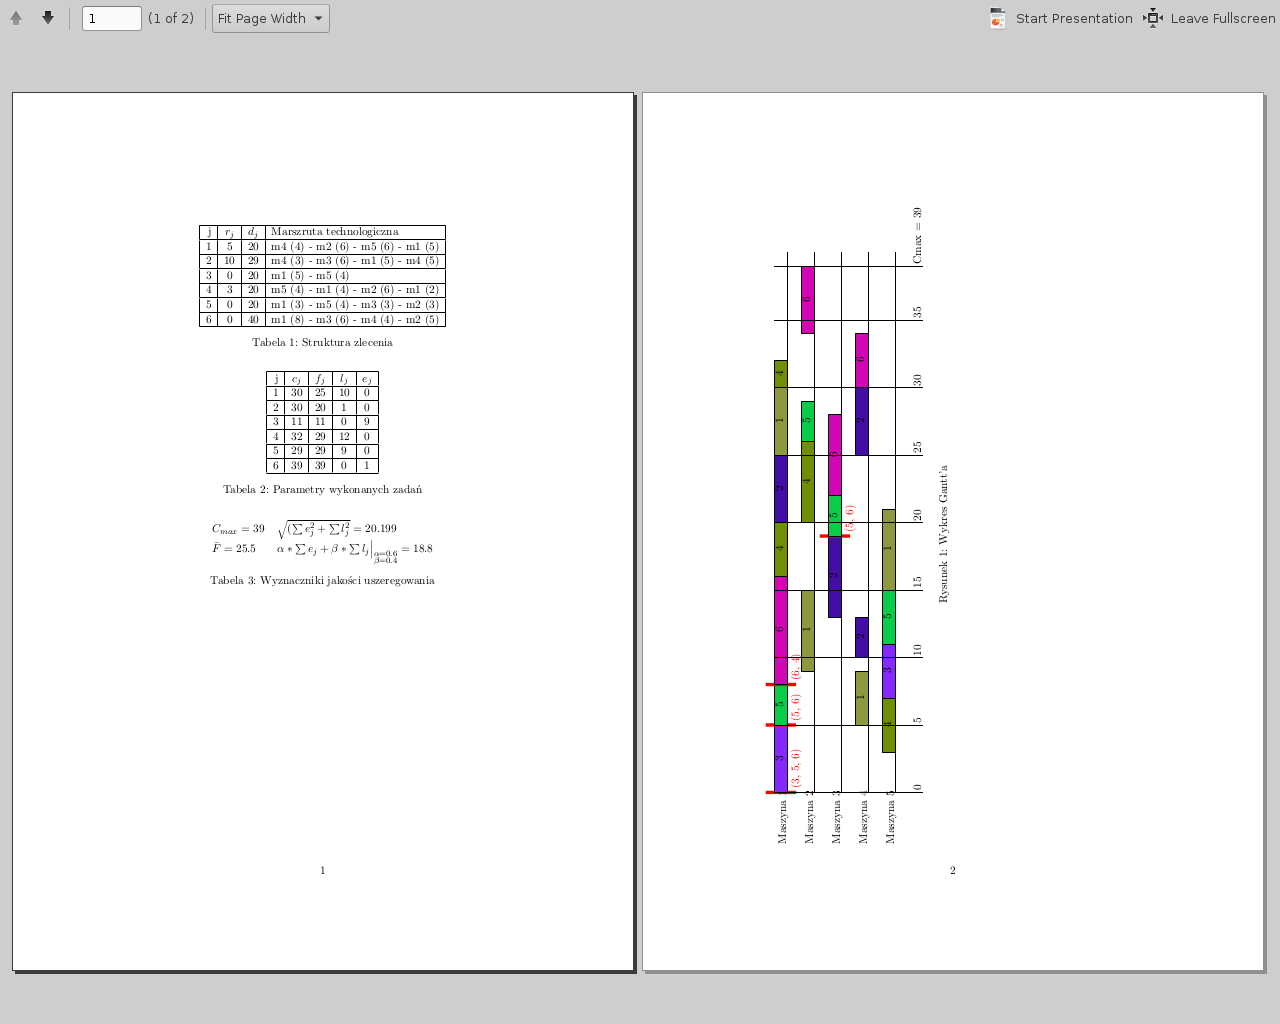
\includegraphics[width=\textwidth, keepaspectratio=true]{./obrazki/pdf}
    \caption{Wyeksportowany plik .pdf}
\end{figure}

Dodatkowo istnieje możliwość obsługi programu kSzereg z poziomu terminalu tekstowego korzystając z wcześniej zapisanych plików .mar, nie jest bowiem możliwa konfiguracja zadaniam jedynie rozwiązanie problemu i eksport wyników do pliku .tex lub .pdf. Zaletą obsługi programu z termianlu jest możliwość podania jako parametr nazwy pliku tekstowego z zapisanymi ścieżkami dostępu do wielu plików .mar, a nawet wybranie obu heurystyk do rozwiązania tych zleceń, co spowoduje rozwiązanie JSSP dla każdego z tych zadań po kolei bez ingerencji użytkownika. Bardziej szczegółowy opis interfejsu lini poleceń jest dostępny po uruchomieniu programu z przełącznikiem '--help'.

\begin{figure}[htb]
    \centering
    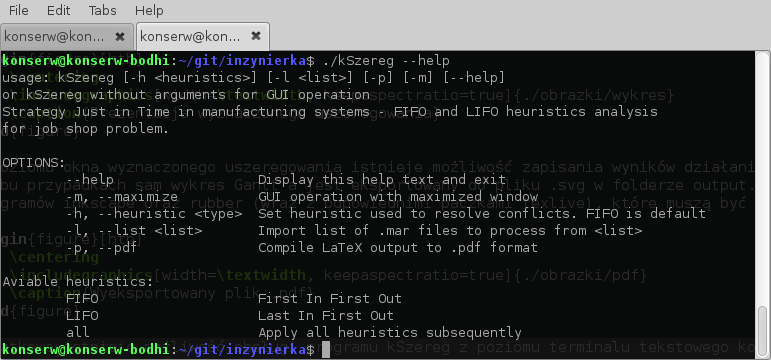
\includegraphics[width=\textwidth, keepaspectratio=true]{./obrazki/cli}
    \caption{Pomoc interface'u linii poleceń}
\end{figure}

   
\section      %  [Przykładowe problemy \ldots]
                {Zastosowanie programu kSzereg}
       
\subsection     {Probelm 1}
\subsubsection  {FIFO}
\input {zad1_FIFO.tex}
\subsubsection  {LIFO}
\input{ zad1_LIFO.tex}

\newpage
\subsection     {Problem 2}
\subsubsection  {FIFO}
\input {zad2_FIFO.tex}
\subsubsection  {LIFO}
\input {zad2_LIFO.tex}

\newpage
\subsection     {Problem 3}
\subsubsection  {FIFO}
\input {zad3_FIFO.tex}
\subsubsection  {LIFO}
\input {zad3_LIFO.tex}

\newpage
\subsection     {Problem 3}
\subsubsection  {FIFO}
\input {zad4_FIFO.tex}
\subsubsection  {LIFO}
\input {zad4_LIFO.tex}

\section        {Wnioski}

%\dodatkowo{Programy}
%tu programy
%\begin{verbatim}
%#include <stdio.h>
%int main()
%{
%   printf("Hello world\n");
%}
%\end{verbatim}              
   
\begin{thebibliography}{99}

%\bibitem{lagrange}
%Lagrangian Bounds for Just-In-Time Job-Shop Scheduling \\
%Philippe Baptiste Marta Flamini Francis Sourd

\bibitem{pastuszak} 
Zarządzanie logistyczne Podstawowe definicje \\
dr Zbigniew Pastuszak

\bibitem{grzechca}
Wykłady z przedmiotu Zautomatyzowane Systemy Wytwarzania\\
dr inż. Waldemar Grzechca na podstawie materiałów prof. dr hab. inż. Mirosława Zaborowskiego \\
Źródło: \url{http://platforma.polsl.pl/rau1} [dostęp:~20.12.12]
\bibitem{wiki}
Linia produkcyjna \\
Źródło: \url{http://pl.wikipedia.org/wiki/Linia_produkcyjna} [dostęp:~20.12.12]

\bibitem{antColony}
Ant Colony Algorithm for Just-in-Time Job Shop Scheduling with Transportation Times and Multirobots \\
Fatima El Khoukhi, Tarik Lamoudan, Jaouad Boukachour, Ahmed El Hilali Alaoui

\bibitem{np}
Algorithms and Theory of Computation Handbook, CRC Press LLC, 1999, "strongly NP-hard", in \href{http://xlinux.nist.gov/dads/}{Dictionary of Algorithms and Data Structures} [online], Paul E. Black, ed., U.S. \href{http://www.nist.gov/}{National Institute of Standards and Technology}. 17 December 2004. Available from: \url{http://www.nist.gov/dads/HTML/stronglyNP.html} [dostęp:~7.01.2013]

\bibitem{genetyczne}
Genetic Algorithm and Local Search for Just-in-Time Job–Shop Scheduling \\
Rodolfo Pereira Araujo, André Gustavo dos Santos, José Elias Cláudio Arroyo \\
2009 IEEE Congress on Evolutionary Computation (CEC 2009)




\end{thebibliography}
\end{document}        
